En annen måte å illustrere transistorens modi på
er ved forholdet mellom spenningene.
\\\\
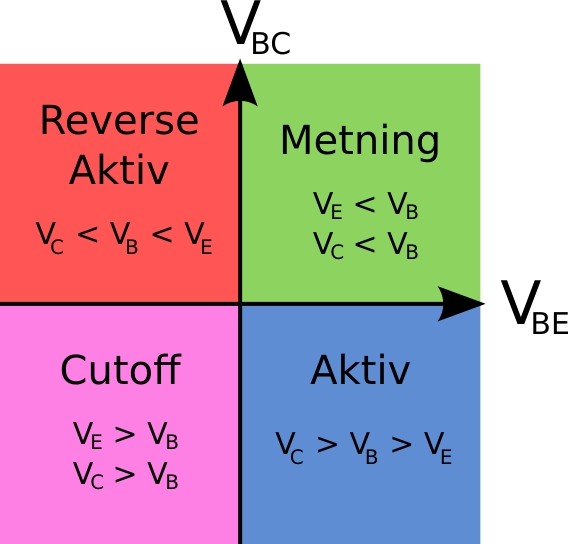
\includegraphics[width=0.5\textwidth]{./img/modi-kvadrant}
\\\\
$V_C = $ spenning fra collector til jord. \\
$V_E = $ spenning fra emitter til jord. \\
$V_B = $ spenning fra base til jord. \\
$V_{BC} = $ spenning fra base til collector. \\
$V_{BE} = $ spenning fra base til emitter. \\
